% common packages, fonts, styles and commands
% unlocalised content
\documentclass[a4paper,9pt]{article}
\usepackage{fontspec}
\usepackage[a4paper,lmargin=2cm,rmargin=2cm,bottom=2cm,top=2cm]{geometry}
\usepackage{multicol}
\usepackage{titling}
\usepackage{fancyhdr}
\usepackage{paralist}
\usepackage{gensymb}

\setmainfont{Roboto Slab Light}

% section without title
\newcommand{\nosection}[1]{%
  \refstepcounter{section}%
  \addcontentsline{toc}{section}{\protect\numberline{\thesection}#1}%
  \markright{#1}}

% title formatting
\newfontfamily\headingfont[]{Oswald}
\newfontfamily\constfont[]{Roboto}
\newcommand{\constt}[1]{{\constfont\selectfont{\textit{#1}}}}
\renewcommand{\maketitlehooka}{\headingfont}
\setlength{\droptitle}{-5em}

% paragraph spacing
\setlength{\parindent}{0em}
\setlength{\parskip}{0.5em}


\usepackage{background}
\usetikzlibrary{calc}
\usepackage{fixltx2e}
\usepackage{unicode-math}
\usepackage{fancybox}
\usepackage{amsmath}
\usepackage{graphicx}
\usepackage{tabularx}

% lines for cutting and bending for folded book like manual
\backgroundsetup{
color=black,
scale=1,
opacity=1,
angle=0,
contents={\tikz\draw[line width=0.1mm, gray]
    (0mm, 0mm) -- (0mm, 297mm)
    (180mm, 0mm) -- (180mm, 297mm)
    [dashed]
    (60mm, 0mm) -- (60mm, 297mm)
    (120mm, 0mm) -- (120mm, 297mm);
  }
}

\newcommand{\makefulltitle}{How To Use The Slide Rule }
% localisation strings used in the templates
\newcommand{\tabstockupper}{Upper half of the Stock }
\newcommand{\tabslidefront}{Front side of the Slide }
\newcommand{\tabslideback}{Reverse side of the Slide }
\newcommand{\tabstocklower}{Lower half of the Stock }
% custom page number
\fancypagestyle{plain}{% title page
  \renewcommand{\headrulewidth}{0pt}%
  \fancyhf{}%
  \fancyfoot[L]{\headingfont{http://wheel.creat.io/sr}}%
  \fancyfoot[R]{\headingfont{\makefulltitle \textbf{\thepage}}}%
  \renewcommand{\headrulewidth}{0pt}
}
\pagestyle{fancy}% other pages
\fancyhf{}
\lfoot{\headingfont{http://wheel.creat.io/sr}}
\rfoot{\headingfont{\makefulltitle \textbf{\thepage}}}
\renewcommand{\headrulewidth}{0pt}


% common part of how-to perex
\newcommand{\makeperex}{Slide Rule is an analog computer, a device that you can use to perform most of the basic and some advanced mathematical operations. It is not as precise and easy to use as pocket calculator, but elegantly demonstrates the laws of mathematics. It is a historical artifact that was still commonly used 50 years ago in many fields of science and technology, engineers and astronauts in space missions used it for flight parameters and trajectory calculations. }
% custom page number
\fancypagestyle{plain}{% title page
  \renewcommand{\headrulewidth}{0pt}%
  \fancyhf{}%
  \fancyfoot[L]{\headingfont{http://wheel.creat.io/sr}}%
  \fancyfoot[R]{\headingfont{\makefulltitle \textbf{\thepage}}}%
  \renewcommand{\headrulewidth}{0pt}
}
\pagestyle{fancy}% other pages
\fancyhf{}
\lfoot{\headingfont{http://wheel.creat.io/sr}}
\rfoot{\headingfont{\makefulltitle \textbf{\thepage}}}
\renewcommand{\headrulewidth}{0pt}





\title{\fontsize{60}{60}\selectfont THE SLIDE RULE}
\preauthor{}\postauthor{}\author{}
\predate{}\postdate{}\date{}
\everymath{\displaystyle}
\begin{document}

  \begin{center}
    \headingfont\fontsize{28}{28}\selectfont HOW TO USE THE SLIDE RULE
  \end{center}

%  {\let\newpage\relax\maketitle}% no new line before title
  \nosection{}
  \large\textbf{\makeperex This guide describes how to use a paper made Slide Rule \modelname.}

  \begin{multicols*}{3}
  \normalsize{
  The Slide Rule consists of three components:
    \begin{inparaenum}[a\upshape)]
      \item Stock;
      \item Slide; and
      \item Cursor.
    \end{inparaenum}

  On the Stock face and both sides of the Slide there are logarithmic scales marked by capital letters:

  % table of stock and slide scales
\renewcommand{\arraystretch}{1.2}
\begin{center}
  \begin{tabular}{ |c|c|}
    \hline
    \multicolumn{2}{|c|}{\tabstockupper} \\
    \hline
      L & \(log x\) \\
    \hline
      P & \(\sqrt{1 - x^2}\) \\
    \hline
      K & \(x^3\) \\
    \hline
      A & \(x^2\) \\
    \hline
    \hline
    \multicolumn{2}{|c|}{\tabslidefront} \\
    \hline
      B & \(x^2\) \\
    \hline
      CI & \(1/x\) \\
    \hline
      C & \(x\) \\
    \hline
    \hline
    \multicolumn{2}{|c|}{\tabslideback} \\
    \hline
      LL1 & \(e^{0.01x}\) \\
    \hline
      LL2 & \(e^{0.1x}\) \\
    \hline
      LL3 & \(e^{1x}\) \\
    \hline
    \hline
    \multicolumn{2}{|c|}{\tabstocklower} \\
    \hline
      D & \(x\) \\
    \hline
      S & \(sin x\) \\
    \hline
      T & \(tan x\) \\
    \hline
      ST & \(sin x \approx tan x \) \\
    \hline
  \end{tabular}
\end{center}


  Lines on the scales are called \textbf{indexes} or divisions. Labels on the scale designate major indexes.

  On the back of the Stock there are located tables of mathematical and physical constants, and other useful graphics\footnote{The metric and inch scales on the back of the Stock and on the front of the Cursor may not be accurate due to temperatures used by the printer and humidity during glueing that alter the paper properties and dimensions.}, but those are not directly involved in calculations. The Slide contains, besides the logarithmic scales on both sides, conversion ratios between imperial and metric (SI) units.

  The Slide slides inside the Stock and the Cursor slides on the top of the Stock. By sliding these parts, aligning the scales at appropriate indexes and reading them, mathematical operations are performed. Some operations require a little deal of mental arithmetic to sort out decimal places.

  \centerline{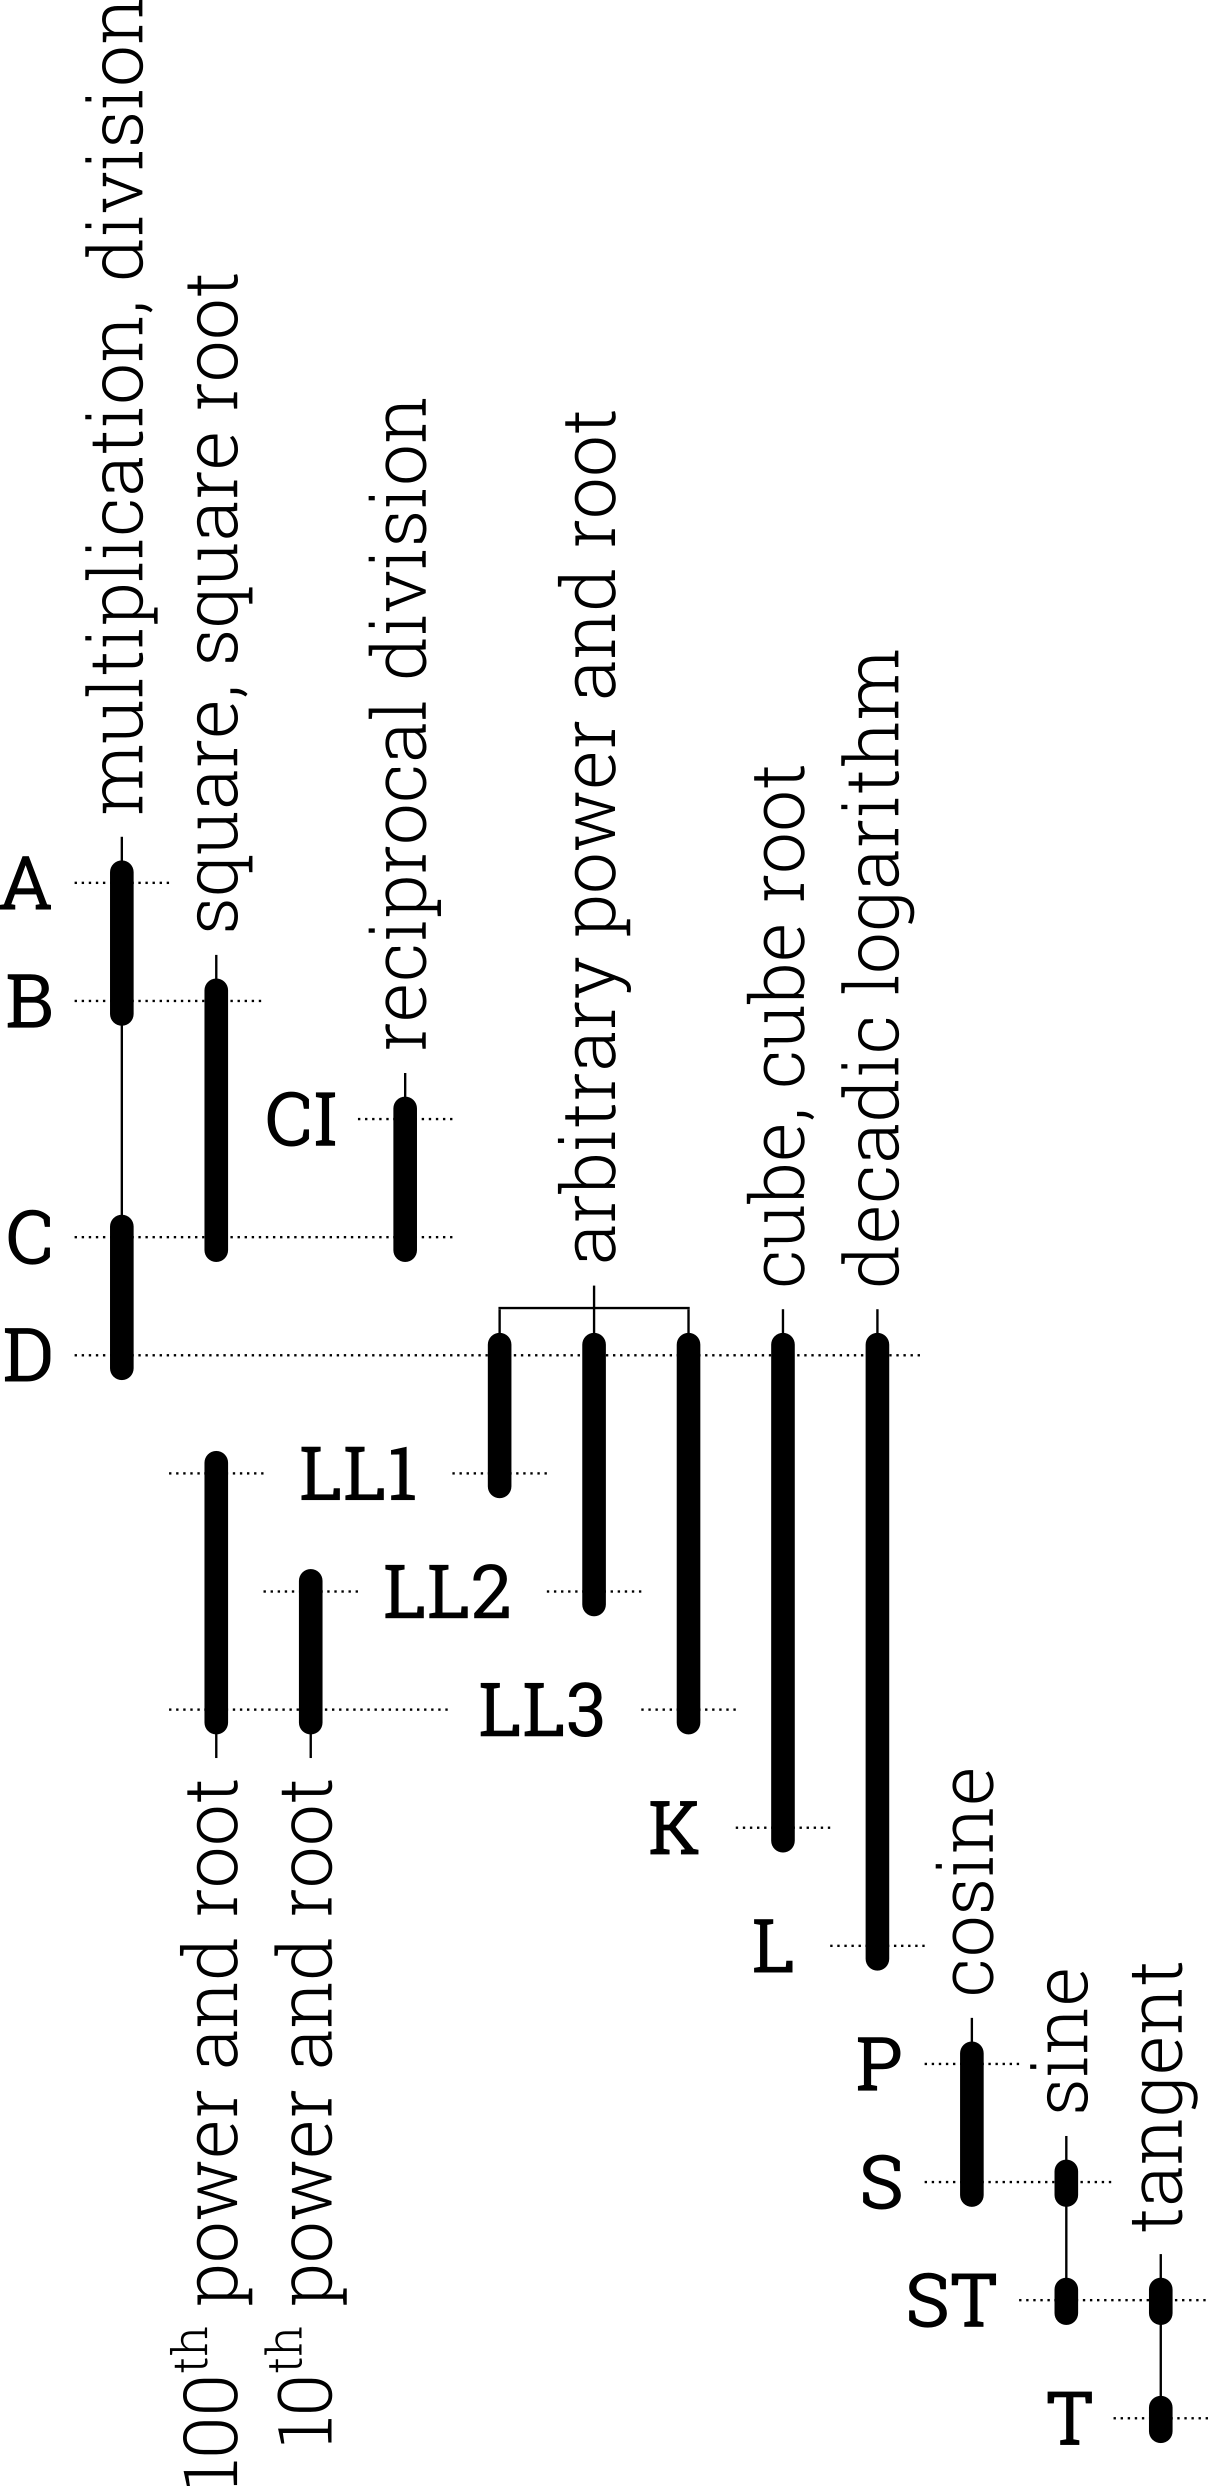
\includegraphics{ops_en}}
  \vspace*{3mm}

  \makeop{2mm}{{x}\cdot{y}}
  \textbf{Basic Multiplication}

\constt{1.2{\char"00D7}2.3:}
Move index 1 on the scale C to position of index 1.2 on the scale D.
Move the Cursor to index 2.3 on scale D.
The position that the Cursor shows on scale C is the result: \constt{2.76}.

\footnotesize Use the scales A and B for multiplication and division of bigger numbers.
\normalsize

  \textbf{Wrap-around Multiplication}

\constt{2.4{\char"00D7}4.6}
Move index 10 on the scale C to 2.4 on the scale D.
Slide the Cursor to index 4.6 on the scale C.
Value on the scale D is is at 1.105.
Mental calculation of approximate values 2.5{\char"00D7}5 gives result of 12.5.
The result is therefore greater than 10.
Adjusting decimal place gives the result: \constt{11.05}. 

  \makeop{2mm}{{x}/{y}}
  \textbf{Basic Division}

\constt{4.6/7.7:}
Move the Cursor index 4.6 on the scale D.
Slide index 7.7 on the scale C to the Cursor.
Move the Cursor to either index 1 or index 10 on the scale C, whichever is in range. In this case, index 10.
The Cursor is now at index 5.97. The correct answer is near 4 / 8 = 0.5. Adjusting decimal place gives the result: \constt{0.597}.

  \makeop{2mm}{{1}/{x}}
  \textbf{Reciprocal Value}

\footnotesize Scale CI is an inverse scale, numbers increase from the right to the left. \normalsize

\constt{1/7.6:}
Move the Cursor to index 7.8 on the scale CI.
The cursor is now at 1.132 on the scale C.
The correct answer is near 1 / 10 = 0.1. Adjusting decimal place gives the result: \constt{0.1132}.

  \makeop{3mm}{x^2}
  \textbf{Square Number}

\constt{4.2\textsuperscript{2}:}
Move the Cursor to index 4.2 on the scale C.
The Cursor is at result index \constt{17.6} on the scale B.

  \makeop{3mm}{\sqrt{x}}
  \textbf{Square Root}

\footnotesize For square root of numbers with odd number of digits, use range [1, 10] on the scale B. For square root of numbers with even number of digits, use range [10, 100] on the scale B. \normalsize

\constt{4400\textsuperscript{0.5}:}
Move the Cursor to index 44 on the scale B (4400 has even number of digits).
The Cursor is at index 6.65 on the scale C. The correct answer is near 70, as 70\textsuperscript{2} = 4900. Adjusting decimal places gives the result: \constt{66.5}.

  \makeop{3mm}{x^3}
  \textbf{Cube}

\constt{4.8\textsuperscript{3}:}
Move the Cursor to index 4.8 on the scale D.
The position of the Cursor on the scale K gives the result: \constt{110}.

  \makeop{3mm}{\sqrt[\leftroot{5}\uproot{2}3]{x}}
  \textbf{Cube Root}

\footnotesize Range [1, 10] on the scale K is used for cube roots of one-digit numbers, range [10, 100] for two-digit numbers, [100, 1000] for three-digit numbers. Four digit numbers again the first range, five digit the second range, etc. \normalsize

\constt{4400\textsuperscript{0.33}:}
Move the Cursor to index 4.4 on the scale K (4400 has 4 digits).
The Cursor is now at 1.655 on the scale D.
The correct answer is between 10 and 20 as 10\textsuperscript{3} = 1000 and 20\textsuperscript{3} = 8000. Adjusting decimal place gives the result: \constt{16.55}.

  \makeop{3mm}{{x}^{10}}
  \textbf{Raising to Power of 10}

\footnotesize Powers of 10 and Arbitrary Powers (including Roots) use LL scales, which are located on the reverse side of the Slide. \normalsize

\constt{1.36\textsuperscript{10}:}
Move the Cursor to index 1.36 on the scale LL2.
The Cursor is now at \constt{21.5} on the scale LL3, which is the result.

  \makeop{3mm}{\sqrt[\leftroot{6}\uproot{2}10]{x}}
  \textbf{10\textsuperscript{th} Root}

\constt{5\textsuperscript{0.1}:}
Move the Cursor to index 5 on the scale LL3.
The Cursor is now at index \constt{1.175} on the scale LL2, which is the result.

  \makeop{3mm}{{x}^{100}}
  \textbf{Raising to Power of 100}

\constt{1.02\textsuperscript{100}:}
Move the Cursor to index 1.02 on the scale LL1.
The Cursor is now at \constt{7.25} on the scale LL3, which is the result.

  \makeop{3mm}{\sqrt[\leftroot{7}\uproot{2}100]{x}}
  \textbf{100\textsuperscript{th} Root}

\constt{5\textsuperscript{0.01}:}
Move the Cursor to index 5 on the scale LL3.
The Cursor is now at index \constt{1.022} on the scale LL1, which is the result.

  \makeop{3mm}{x^y}
  \textbf{Arbitrary Power}

\constt{9.1\textsuperscript{2.3}:}
Move index 9.1 on the scale LL3 to the position of index 1 on the scale D.
Move the Cursor to index 2.3 on the scale D.
The position of the Cursor on the scale LL3 shows the result: \constt{160.6}. The Cursor is actually about 161, the scale loses precision with increasing range. 

\constt{230\textsuperscript{0.45}:}
Move index 230 on the scale LL3 to the position of index 10 on the scale C.
Move the Cursor to index 4.5 on the scale C.
The Cursor is now at index \constt{11.6} on the scale LL3, which is the result.

\constt{0.78\textsuperscript{3.4}:}
Move index 3.4 on the scale LL3 to the position of index 7.8 on the scale C.
Move the Cursor to index 10 on the scale C.
The Cursor is now at index \constt{4.3} on the scale LL3, which is the result.

\constt{1.9\textsuperscript{2.5}:}
Move index 1.9 on the scale LL2 to the position of index 10 on the scale C.
Move the Cursor to index 2.5 on the scale C.
The Cursor is now at position \constt{4.97} on the scale LL3, which is the result.

\constt{0.99\textsuperscript{560}:}
Move index 9.9 on the scale LL3 to the position of index 10 on the scale C.
Move the Cursor to index 5.6 on the scale C.
The Cursor is now at index 3.6 on the scale LL3.
As we used one 100\textsuperscript{th} of the exponent, we adjust the value by two decimal places, which gives the result: \constt{0.036}.

  \makeop{3mm}{\sin{x}}
  \textbf{Sine}

\footnotesize Use scale S for finding sine of angles between 5\textdegree and 90\textdegree, and scale ST for angles between 30' and 6\textdegree. \normalsize

\constt{sin(33\textdegree):}
Move the Cursor to index 33 on the scale S.
The Cursor is at index 5.45 on the scale C.
The correct answer is between 0.1 and 1. Adjusting decimal place gives the result: \constt{0.545}.

  \makeop{3mm}{\cos{x}}
  \textbf{Cosine}

\constt{cos(33\textdegree):}
Move the Cursor to index 33 on the scale S.
The Cursor is at index \constt{0.83} on the scale P (it is an inverse scale), which gives the result.

  \makeop{3mm}{\tan{x}}
  \textbf{Tangent}

\footnotesize Use scale T for finding tangent of angles between 5\textdegree and 45\textdegree, and scale ST for angles between 30' and 6\textdegree. \normalsize

\constt{tan(33\textdegree):}
Move the Cursor to index 33 on the scale S.
The Cursor is at index 6.5 on the scale D.
The correct answer is between 0.1 and 1. Adjusting decimal place gives the result: \constt{0.65}.

  \makeop{3mm}{\log_{10}{x}}
  \textbf{Logarithm of Base 10}

\constt{log\textsubscript{10}2.6:}
Move the Cursor to index 2.6 on the scale C.
The Cursor is now at index 4.14 on the scale L.
Adjusting decimal place gives the result: \constt{0.414}.
  }
  \end{multicols*}
  
\end{document}
